\documentclass[11pt]{beamer}
\usetheme{Berlin}
\usepackage[utf8]{inputenc}
\usepackage[english]{babel}
\usepackage{amsmath}
\usepackage{amsfonts}
\usepackage{amssymb}
\usepackage{graphicx}
\usepackage{xcolor}
\usepackage{booktabs}
\author{Adam Aili \& Erik Ekelund}
\title{Half-time report}
%\setbeamercovered{transparent} 
\setbeamertemplate{navigation symbols}{} 
%\logo{} 
%\institute{} 
\date{\today} 
%\subject{} 
\beamerdefaultoverlayspecification{<+->}
\begin{notation}% Passing the option "old" to the notation environment will redefine the notationtabular environment so that it produces an old style LaTeX tabular instead of a ctable.sty style tabular.
  \centering
  
% Lägg in förkortningarna i bokstavsordning!
  \begin{notationtabular}{Abbreviations}{Abbreviation}{Description}
    \abbrCB\index{CB@\abbrCG!abbreviation} & Center of buoyancy. \\
    \abbrCG\index{CG@\abbrCG!abbreviation} & Center of gravity. \\
    \abbrCO\index{CO@\abbrCO!abbreviation} & Center of origin. \\
    \abbrDOF\index{DOF@\abbrDOF!abbreviation} & Degrees of freedom. \\
    \abbrEKF\index{EKF@\abbrEKF!abbreviation} & Extended Kalman filter.\\
    \abbrESC\index{ESC@\abbrESC!abbreviation} & Electronic speed controller.\\
    \abbrIMU\index{IMU@\abbrIMU!abbreviation} & Inertial measurement unit.\\
    \abbrIO\index{I/O@\abbrIO!abbreviation}   & Input/Output.\\
    \abbrKF\index{KF@\abbrKF!abbreviation}	& Kalman filter.\\
    \abbrMPC\index{MPC@\abbrMPC!abbreviation} & Model predictive control.\\
    \abbrPID\index{PID@\abbrPID!abbreviation} & Proportional, integral, differential (regulator). \\
    \abbrPI\index{PI@\abbrPI!abbreviation} & Proportional, integral (regulator). \\
    \abbrRPM\index{RPM@\abbrRPM!abbreviation} & Rotations per minute. \\
    \abbrSLAM\index{SLAM@\abbrSLAM!abbreviation} & Simultaneous localisation and mapping. \\
    \abbrSNR\index{SNR@\abbrSNR!abbreviation} & Signal to noise ratio. \\
    \abbrROS\index{ROS@\abbrROS!abbreviation} & Robot Operating System. \\
    \abbrROV\index{ROV@\abbrROV!abbreviation} & Remotely operated vehicle. \\
    \abbrUV\index{UV@\abbrUV!abbreviation} & Unmanned vehicle. \\

    
    
  \end{notationtabular}
  
\end{notation}


\begin{document}


\begin{frame}
\titlepage
\end{frame}

\begin{frame}{Outline}
\tableofcontents
\end{frame}

\section{Software}
\begin{frame}{Controllers}


\end{frame}

\begin{frame}{Sensor fusion}


\end{frame}

\begin{frame}{Arduino}
\begin{itemize}
\item HMC5883L - Magnetometer
\item MS5611 - Barometer
\item MPU6000 - IMU
\item MS5837-30BA - Pressure sensor
\end{itemize}
\end{frame}

\section{ROV Assembly}
\begin{frame}{}

\end{frame}

\section{Parameter Estimation}
\begin{frame}[shrink]{Translation dynamics}
\begin{multline} \label{eq:u_dot}
\dot{u} = \frac{\thrusterfun{3} + \thrusterfun{4}}{m -\Xudot} + \frac{u (\Xu + \Xuabsu \abs{u})}{m -\Xudot} + \frac{\sin(\theta)(B - W)}{m -\Xudot} +
\frac{m(r v - q w )}{m -\Xudot} + \\ \frac{-\Yvdot r v}{m -\Xudot} + \frac{\Zwdot q w}{m -\Xudot},
\end{multline}
\begin{multline} \label{eq:v_dot}
\dot{v} = \frac{-\thrusterfun{6}}{m - \Yvdot} + \frac{v (\Yv + \Yvabsv \abs{v})}{m - \Yvdot} + \frac{-\cos{\theta} \sin{\phi}(B - W)}{m - \Yvdot} +\\ \frac{m(p w - r u)}{m - \Yvdot} + \frac{\Xudot r u}{m - \Yvdot} + \frac{-\Zwdot p w}{m - \Yvdot},
\end{multline}
\begin{multline} \label{eq:w_dot}
\dot{w} = \frac{-\thrusterfun{1} - \thrusterfun{2} - \thrusterfun{5}}{m - \Zwdot} + \frac{w (\Zw + \Zwabsw \abs{w})}{m - \Zwdot} + \frac{-\cos{\phi}\cos{\theta}(B - W)}{m - \Zwdot} +\\
\frac{m (q u - p v)}{m - \Zwdot} + \frac{-\Xudot q u}{m - \Zwdot} + \frac{\Yvdot p v}{m - \Zwdot},
\end{multline}
\end{frame}

\begin{frame}[shrink]{Rotational dynamics}
\begin{multline} \label{eq:p_dot}
\dot{p} = \frac{\thrusterfun{1} \distance{y}{1} - \thrusterfun{2} \distance{y}{2} + \thrusterfun{6} \distance{z}{6}}{\Ix - \Kpdot} + \frac{p (Kp + \Kpabsp \abs{p})}{\Ix - \Kpdot} + \frac{-\Mqdot q r}{\Ix - \Kpdot} + \frac{\Nrdot q r}{\Ix - \Kpdot} +\\
\frac{q r (\Iy - \Iz)}{\Ix - \Kpdot} + \frac{- \Yvdot v w}{\Ix - \Kpdot} + \frac{\Zwdot v w}{\Ix - \Kpdot} + \frac{B \cos{\theta} \sin{\phi} z_B}{\Ix - \Kpdot}
\end{multline},
\begin{multline} \label{eq:q_dot}
\dot{q} =\frac{\thrusterfun{1} \distance{x}{1} + \thrusterfun{2} \distance{x}{2} - \thrusterfun{5} \distance{x}{5}}{\Iy - \Mqdot} + \frac{q (\Mq + \Mqabsq \abs{q})}{\Iy - \Mqdot} + \frac{\Kpdot p r}{\Iy - \Mqdot} + \frac{-\Nrdot p r}{\Iy - \Mqdot} +\\
\frac{p r (\Iz - \Ix)}{\Iy - \Mqdot} + \frac{-\Zwdot u w}{\Iy - \Mqdot} + \frac{\Xudot u w}{\Iy - \Mqdot} + \frac{B \sin{\theta} z_B}{\Iy - \Mqdot} 
\end{multline},
\begin{multline} \label{eq:r_dot}
\dot{r} = \frac{\thrusterfun{3} \distance{y}{3} - \thrusterfun{4} \distance{y}{4}}{\Iz - \Nrdot} + \frac{r (\Nr + \Nrabsr \abs{r})}{\Iz - \Nrdot} + \frac{-\Kpdot p q}{\Iz - \Nrdot} + \frac{\Mqdot p q}{\Iz - \Nrdot} +\\
\frac{p q (\Ix - \Iy)}{\Iz - \Nrdot} + \frac{- \Xudot u v}{\Iz - \Nrdot} + \frac{\Yvdot u v}{\Iz - \Nrdot}
\end{multline} 
\end{frame}

\begin{frame}[shrink]{Roll and Pitch}
\begin{multline*}
\dot{p} = \frac{\thrusterfun{1} \distance{y}{1} - \thrusterfun{2} \distance{y}{2} + \thrusterfun{6} \distance{z}{6}}{\Ix - \Kpdot} + \frac{p (Kp + \Kpabsp \abs{p})}{\Ix - \Kpdot} + \frac{-\Mqdot q r}{\Ix - \Kpdot} + \\ \frac{\Nrdot q r}{\Ix - \Kpdot} + \frac{q r (\Iy - \Iz)}{\Ix - \Kpdot} + \textcolor{red}{\frac{- \Yvdot v w}{\Ix - \Kpdot} + \frac{\Zwdot v w}{\Ix - \Kpdot}} + \frac{B \cos{\theta} \sin{\phi} z_B}{\Ix - \Kpdot}
\end{multline*}
\begin{multline*}
\dot{q} =\frac{\thrusterfun{1} \distance{x}{1} + \thrusterfun{2} \distance{x}{2} - \thrusterfun{5} \distance{x}{5}}{\Iy - \Mqdot} + \frac{q (\Mq + \Mqabsq \abs{q})}{\Iy - \Mqdot} + \frac{\Kpdot p r}{\Iy - \Mqdot} +\\ \frac{-\Nrdot p r}{\Iy - \Mqdot} + \frac{p r (\Iz - \Ix)}{\Iy - \Mqdot} + \textcolor{red}{\frac{-\Zwdot u w}{\Iy - \Mqdot} + \frac{\Xudot u w}{\Iy - \Mqdot}} + \frac{B \sin{\theta} z_B}{\Iy - \Mqdot} 
\end{multline*}
\end{frame}

\begin{frame}{Roll and Pitch}
BILD FRAN COMPARE
\end{frame}

\begin{frame}{Yaw}
\begin{multline*}
\dot{r} = \frac{\thrusterfun{3} \distance{y}{3} - \thrusterfun{4} \distance{y}{4}}{\Iz - \Nrdot} + \frac{r (\Nr + \Nrabsr \abs{r})}{\Iz - \Nrdot} + \frac{-\Kpdot p q}{\Iz - \Nrdot} + \frac{\Mqdot p q}{\Iz - \Nrdot} +\\
\frac{p q (\Ix - \Iy)}{\Iz - \Nrdot} + \textcolor{red}{\frac{- \Xudot u v}{\Iz - \Nrdot} + \frac{\Yvdot u v}{\Iz - \Nrdot}}
\end{multline*} 
\end{frame}

\begin{frame}{Yaw}
\begin{figure}
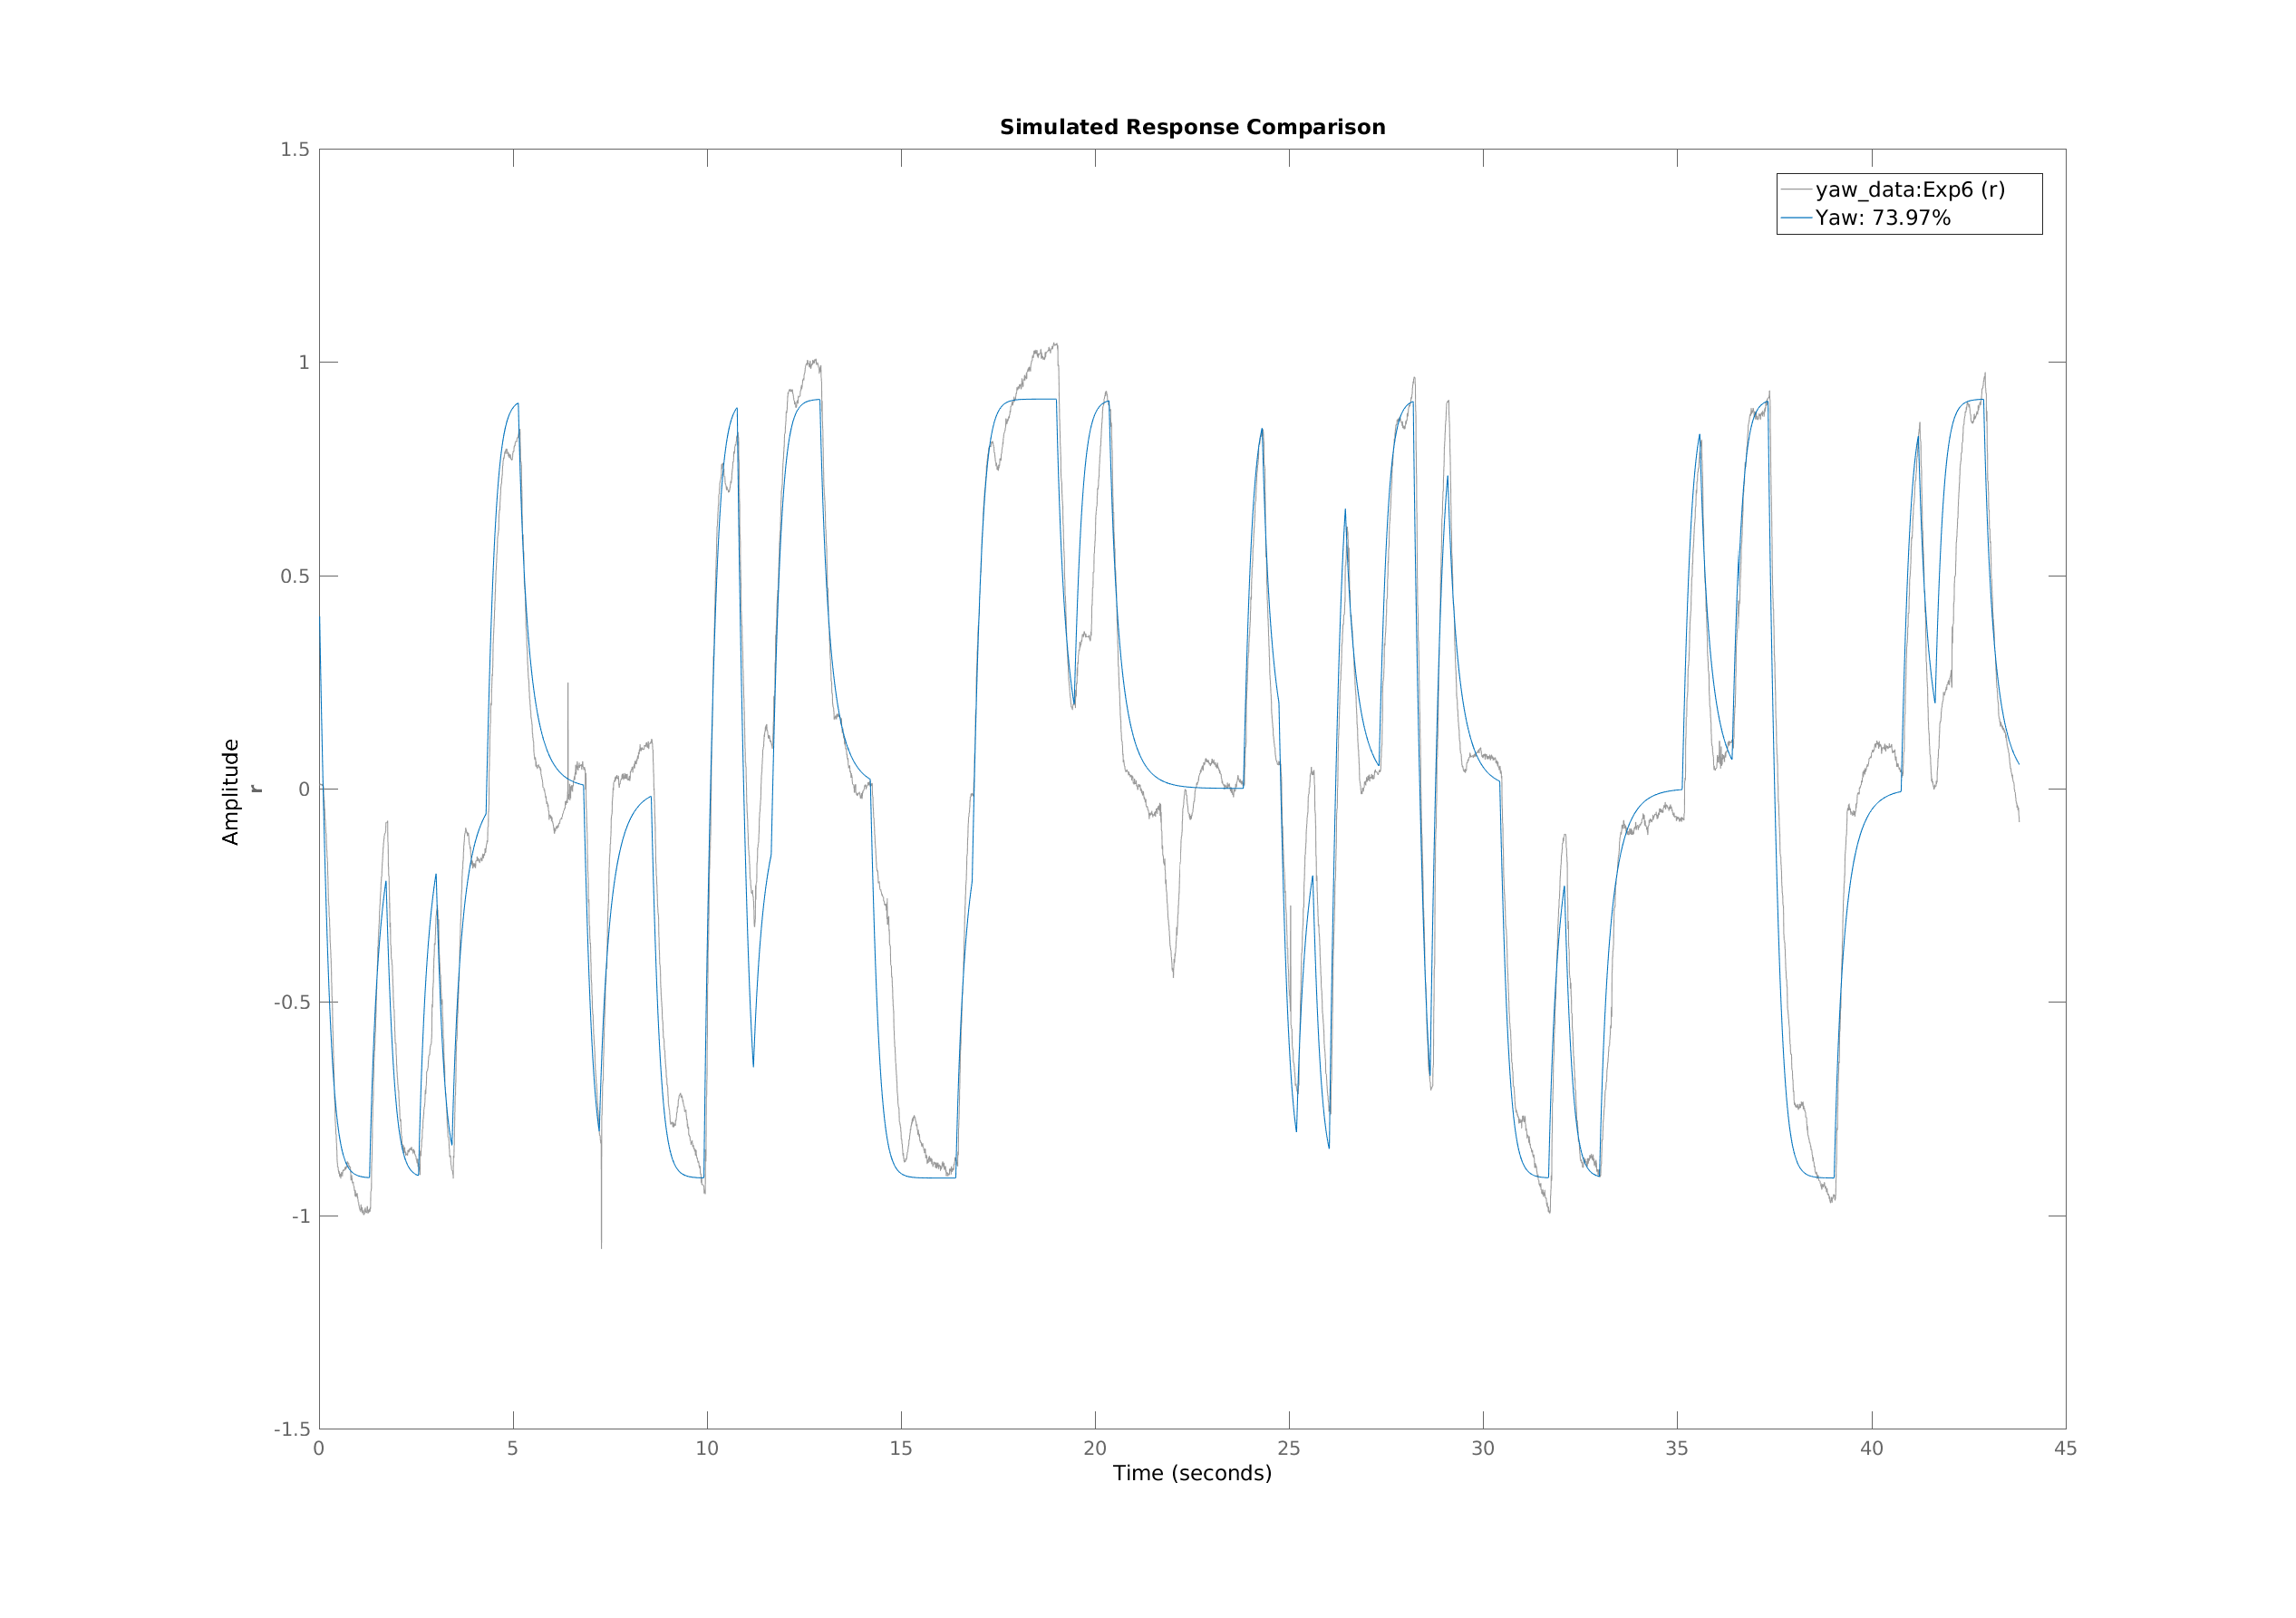
\includegraphics[width=0.9\textwidth]{fig/compareYaw}
\end{figure}
\end{frame}

\begin{frame}{Yaw}
\begin{table}
\begin{tabular}{l l}
\toprule
\textbf{Parameters} & \textbf{Values}\\
\midrule
\Kpdot 	& -1.8347 	\\       
\Mqdot 	& -0.85157	\\        
\Nr    	& -1.344    	\\    
\Nrdot 	& -0.27111  	\\     
\Nrabsr & -1.0733   	\\    
\Ix     &  1.8347   	\\     
\Iy     &  0.85157	\\       
\Iz     &  0.27111  	\\ 
\bottomrule
\end{tabular}
\caption{Estimated yaw parameters}
\end{table}
\end{frame}

\begin{frame}
\begin{columns}[c] 
\column{.45\textwidth} 
\begin{table}
\begin{tabular}{l l}
\toprule
\textbf{Parameters} & \textbf{Values}\\
\midrule
\Kpdot 	& -1.8347 	\\       
\Mqdot 	& -0.85157	\\        
\Nr    	& -1.344    	\\    
\Nrdot 	& -0.27111  	\\     
\Nrabsr & -1.0733   	\\    
\Ix     &  1.8347   	\\     
\Iy     &  0.85157	\\       
\Iz     &  0.27111  	\\ 
\bottomrule
\end{tabular}
\caption{Estimated yaw parameters}
\end{table}

\column{.5\textwidth}
\begin{table}
\begin{tabular}{l l}
\toprule
\textbf{Parameters} & \textbf{Values}\\
\midrule
\bottomrule
\end{tabular}
\caption{Estimated roll and pitch parameters}
\end{table}
\end{columns}
\end{frame}

\section{Simulation}
\begin{frame}{}

\end{frame}

\section{Controllers}
\begin{frame}{}

\end{frame}

\section{Future Work}
\begin{frame}{}

\end{frame}

\end{document}